\chapter{Implementacija i korisničko sučelje}
		
		
		\section{Korištene tehnologije i alati}
		
			\textbf{\textit{dio 2. revizije}}
			
			 \textit{Detaljno navesti sve tehnologije i alate koji su primijenjeni pri izradi dokumentacije i aplikacije. Ukratko ih opisati, te navesti njihovo značenje i mjesto primjene. Za svaki navedeni alat i tehnologiju je potrebno \textbf{navesti internet poveznicu} gdje se mogu preuzeti ili više saznati o njima}.
			
			
			\eject 
		
	
		\section{Ispitivanje programskog rješenja}
			
			\textbf{\textit{dio 2. revizije}}\\
			
			 \textit{U ovom poglavlju je potrebno opisati provedbu ispitivanja implementiranih funkcionalnosti na razini komponenti i na razini cijelog sustava s prikazom odabranih ispitnih slučajeva. Studenti trebaju ispitati temeljnu funkcionalnost i rubne uvjete.}
	
			
			\subsection{Ispitivanje komponenti}
			\textit{Potrebno je provesti ispitivanje jedinica (engl. unit testing) nad razredima koji implementiraju temeljne funkcionalnosti. Razraditi \textbf{minimalno 6 ispitnih slučajeva} u kojima će se ispitati redovni slučajevi, rubni uvjeti te izazivanje pogreške (engl. exception throwing). Poželjno je stvoriti i ispitni slučaj koji koristi funkcionalnosti koje nisu implementirane. Potrebno je priložiti izvorni kôd svih ispitnih slučajeva te prikaz rezultata izvođenja ispita u razvojnom okruženju (prolaz/pad ispita). }
			
			 

			\subsection{Ispitivanje sustava}
Ispitivanje sustava ostvareno je Selenium WebDriverom u Pythonu. Provedeni testovi s kodom priloženi su u nastavku.
\break
Prvi ispitni slučaj obrađuje pokušaj prijave emailom koji ne postoji u sustavu. Očekivani izlaz je neuspjeh prijave.

\lstset{language=Python, xleftmargin=0pt}
\begin{lstlisting}
def test1() -> bool:
    url = "http://localhost:3000/login"
    driver.get(url)
    driver.find_element(By.ID, "email").send_keys("osoba@osoba.com")
    driver.find_element(By.ID, "password").send_keys("123456")
    driver.find_element(By.CSS_SELECTOR, "button[type='submit']").click()

    if driver.current_url.endswith("/login"):
        return True
    else:
        return False
\end{lstlisting}

Drugi ispitni slučaj obrađuje pokušaj registracije s emailom u neispravnom formatu. Očekivani izlaz je neuspjeh registracije.

\lstset{language=Python, xleftmargin=0pt}
\begin{lstlisting}
def test2() -> bool:
    url = "http://localhost:3000/login"
    driver.get(url)
    driver.find_element(By.CSS_SELECTOR, "button[type='button']").click()
    driver.find_element(By.ID, "firstname").send_keys("Osoba")
    driver.find_element(By.ID, "lastname").send_keys("Osoba")
    driver.find_element(By.ID, "email").send_keys("osoba.com")
    driver.find_element(By.CSS_SELECTOR, "button[type='submit']").click()

    if driver.current_url.endswith("/register"):
        return True
    else:
        return False
\end{lstlisting}

Treći ispitni slučaj obrađuje pokušaj registracije s svim valjanim podacima. Očekivani izlaz je uspješna registracija i preusmjeravanje.

\lstset{language=Python, xleftmargin=0pt}
\begin{lstlisting}
def test3() -> bool:
    url = "http://localhost:3000/login"
    driver.get(url)
    driver.find_element(By.CSS_SELECTOR, "button[type='button']").click()
    driver.find_element(By.ID, "firstname").send_keys("Osoba")
    driver.find_element(By.ID, "lastname").send_keys("Osoba")
    driver.find_element(By.ID, "email").send_keys("osoba@osoba.com")
    driver.find_element(By.CSS_SELECTOR, "button[type='submit']").click()

    if driver.current_url.endswith("/register"):
        return False
    else:
        return True
\end{lstlisting}

Četvrti ispitni slučaj obrađuje pokušaj prijave s postojećim emailom, ali s neispravnom lozinkom. Očekivani izlaz je neuspjeh prijave.

\lstset{language=Python, xleftmargin=0pt}
\begin{lstlisting}
def test4() -> bool:
    url = "http://localhost:3000/login"
    driver.get(url)
    driver.find_element(By.ID, "email").send_keys("admin@admin.com")
    driver.find_element(By.ID, "password").send_keys("123456")
    driver.find_element(By.CSS_SELECTOR, "button[type='submit']").click()

    if driver.current_url.endswith("/login"):
        return True
    else:
        return False
\end{lstlisting}

Peti ispitni slučaj obrađuje pokušaj prijave s ispravnim emailom i lozinkom. Očekivani izlaz je uspješna prijava i preusmjeravanje. 

\lstset{language=Python, xleftmargin=0pt}
\begin{lstlisting}
def test5() -> bool:
    url = "http://localhost:3000/login"
    driver.get(url)
    driver.find_element(By.ID, "email").send_keys("admin@admin.com")
    driver.find_element(By.ID, "password").send_keys("progi123")
    driver.find_element(By.CSS_SELECTOR, "button[type='submit']").click()
    time.sleep(0.5)

    if driver.current_url.endswith("/login"):
        return False
    else:
        return True
\end{lstlisting}

Na slici 5.1 prikazan je screenshot terminala nakon pokretanja navedenih pet ispitnih slučajeva.

\begin{figure}[htp]
    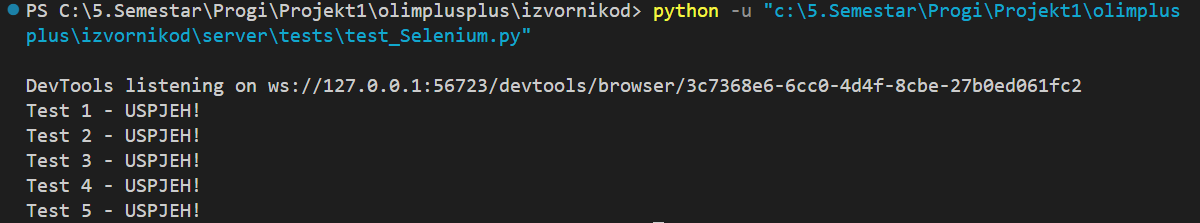
\includegraphics[scale=0.5]{dijagrami/testsScreenshot.png}
    \centering
    \caption{Rezultati ispitivanja Selenium WebDriverom}
\end{figure}

\eject

		
		\section{Dijagram razmještaja}
			
		\begin{figure}[htp]
			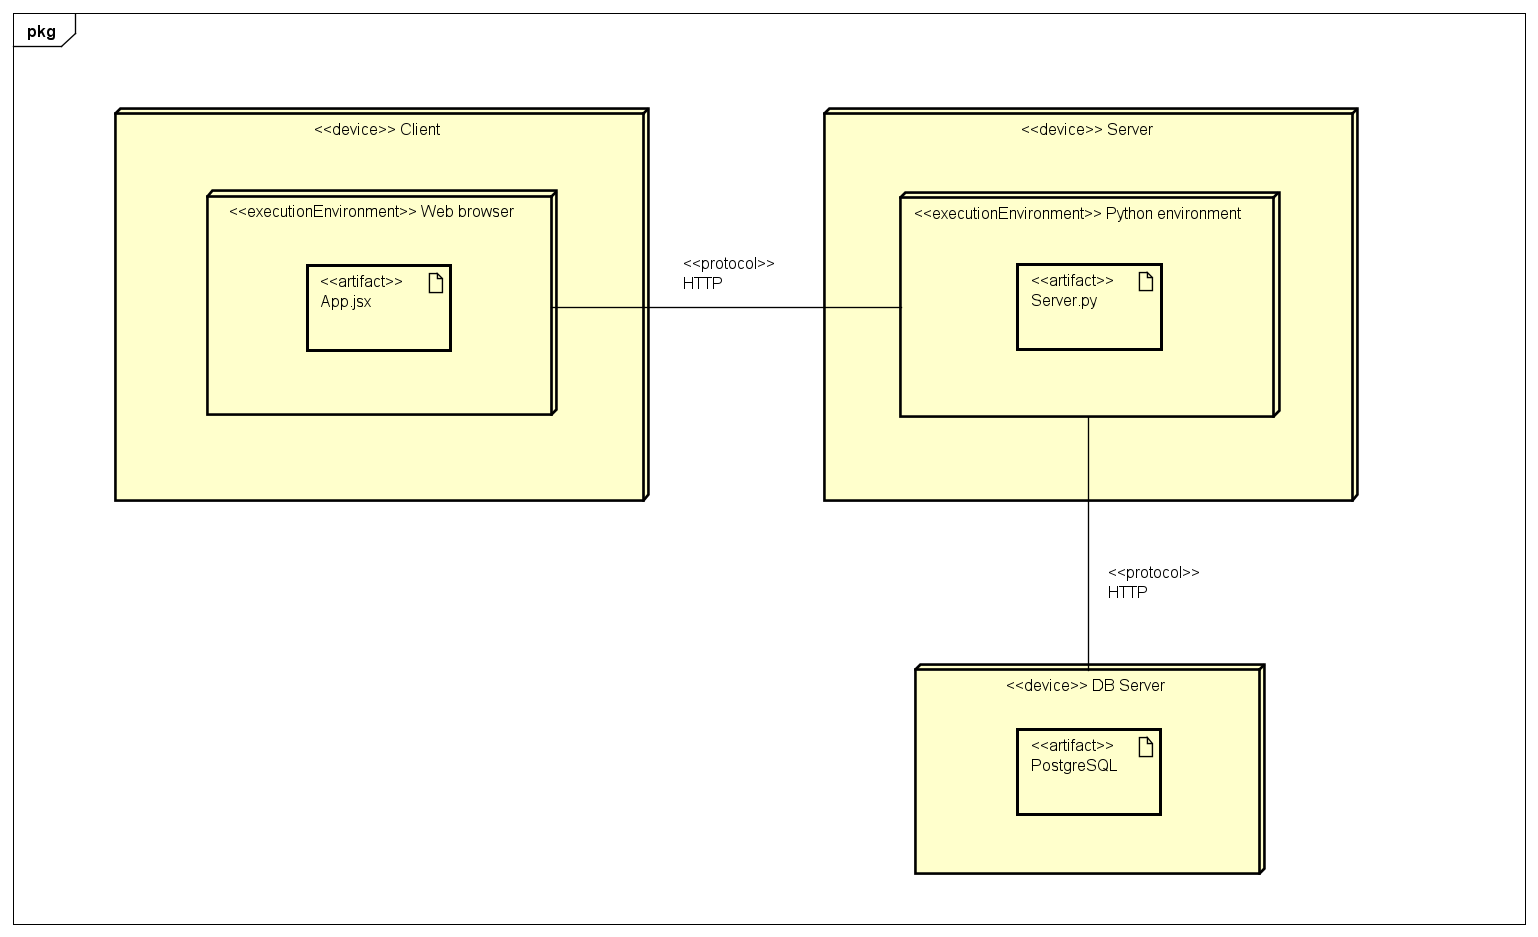
\includegraphics[scale=0.4]{dijagrami/DeploymentDiagram0.png}
			\centering
			\caption{Dijagram razmještaja}
		\end{figure}
		
		\section{Upute za puštanje u pogon}
		
			\textbf{\textit{dio 2. revizije}}\\
		
			 \textit{U ovom poglavlju potrebno je dati upute za puštanje u pogon (engl. deployment) ostvarene aplikacije. Na primjer, za web aplikacije, opisati postupak kojim se od izvornog kôda dolazi do potpuno postavljene baze podataka i poslužitelja koji odgovara na upite korisnika. Za mobilnu aplikaciju, postupak kojim se aplikacija izgradi, te postavi na neku od trgovina. Za stolnu (engl. desktop) aplikaciju, postupak kojim se aplikacija instalira na računalo. Ukoliko mobilne i stolne aplikacije komuniciraju s poslužiteljem i/ili bazom podataka, opisati i postupak njihovog postavljanja. Pri izradi uputa preporučuje se \textbf{naglasiti korake instalacije uporabom natuknica} te koristiti što je više moguće \textbf{slike ekrana} (engl. screenshots) kako bi upute bile jasne i jednostavne za slijediti.}
			
			
			 \textit{Dovršenu aplikaciju potrebno je pokrenuti na javno dostupnom poslužitelju. Studentima se preporuča korištenje neke od sljedećih besplatnih usluga: \href{https://aws.amazon.com/}{Amazon AWS}, \href{https://azure.microsoft.com/en-us/}{Microsoft Azure} ili \href{https://www.heroku.com/}{Heroku}. Mobilne aplikacije trebaju biti objavljene na F-Droid, Google Play ili Amazon App trgovini.}
			
			
			\eject 